\documentclass[coursework]{SCWorks}
% Тип обучения (bachelor), форма (och), тип работы (coursework) по умолчанию

\usepackage{preamble}

% Настройка minted для C++ согласно требованиям и лекциям
\setminted[cpp]{
    frame=lines,
    framesep=2mm,
    baselinestretch=1.2,
    bgcolor=lightgray!10,
    fontsize=\small,
    linenos=true
}

\begin{document}

% Кафедра (в родительном падеже)
\chair{информатики и программирования}

% Тема работы
\title{Применение методов машинного обучения и классификации данных}

% Курс и группа
\course{1}
\group{151}

% Направление подготовки
\napravlenie{09.03.04 "--- Программная инженерия}

% Фамилия, имя, отчество в родительном падеже
\author{Андриянова Афанасия Валерьевича}

% Заведующий кафедрой 
\chtitle{доцент, к.\,ф.-м.\,н.}
\chname{С.\,В.\,Миронов}

% Научный руководитель
\satitle{доцент, к.\,ф.-м.\,н.}
\saname{Г.\,Г.\,Наркайтис}

\maketitle

% Включение нумерации рисунков, формул и таблиц по разделам
\secNumbering

\tableofcontents

% Введение
\intro
В данной работе рассматривается применение современных алгоритмов и подходов для анализа данных и автоматизации вычислений. В качестве демонстрации базовых возможностей системы \LaTeX{} здесь реализованы нормативные требования по внедрению математических выражений, табличных структур, графических зависимостей и листингов программного кода на языке \texttt{C++}.

Актуальность автоматизации подобных отчётов и применения математического моделирования подтверждается во многих современных исследованиях, например, в области анализа аудиоданных~\cite{human_earing} и фундаментальных основ нейросетевых архитектур~\cite{attention}.

% Основная часть (разделенная на логические файлы)
\section{Теоретическая часть и математические основы}

Рассмотрим базовые математические закономерности, используемые при анализе данных. Первой важной формулой является фундаментальное тождество Эйлера, связывающее пять ключевых математических констант:
\begin{equation}
\label{eq:euler}
e^{i\pi} + 1 = 0
\end{equation}

Далее определим функцию нормального распределения вероятностей (кривая Гаусса), которая повсеместно применяется при статистическом анализе данных и в машинном обучении~\cite{henrick2017ml}. Плотность распределения имеет вид:
\begin{equation}
\label{eq:gauss}
f(x) = \frac{1}{\sigma \sqrt{2\pi}} \exp\left( -\frac{1}{2}\left(\frac{x-\mu}{\sigma}\right)^{\!2} \, \right)
\end{equation}

Для оценки итерационных процессов алгоритмов нам потребуется аппарат дискретных сумм. Запишем формулу суммы первых $n$ натуральных чисел:
\begin{equation}
\label{eq:sum}
\sum_{i=1}^{n} i = \frac{n(n+1)}{2}
\end{equation}

Все три формулы "--- \eqref{eq:euler}, \eqref{eq:gauss} и \eqref{eq:sum} "--- являются классическими примерами математического анализа и широко используются при проектировании сложных вычислительных систем.

\subsection{Сводные аналитические данные}

В таблице~\ref{tab:metrics} приведены результаты сравнительного анализа производительности алгоритмов при изменении управляющей переменной \texttt{N}.

\begin{table}[htbp]
    \centering
    \caption{Сравнение времени работы алгоритмов вычислений}
    \label{tab:metrics}
    \begin{tabular}{ccc}
        \hline
        Размерность (\texttt{N}) & Алгоритм А (сек) & Алгоритм Б (сек) \\
        \hline
        100  & 0.001 & 0.002 \\
        1000 & 0.015 & 0.008 \\
        5000 & 0.421 & 0.095 \\
        \hline
    \end{tabular}
\end{table}
\section{Программная реализация алгоритма и визуализация}

Для автоматизации расчетов и генерации данных, частично представленных в таблице~\ref{tab:metrics}, использовался программный модуль, разработанный на языке \texttt{C++}. Ниже представлен листинг~\ref{code:cpp_script}, загруженный напрямую из файла проекта с помощью возможностей пакета \texttt{minted}.

\inputminted[label=script.cpp]{cpp}{script.cpp}
\label{code:cpp_script}

В коде функция \mintinline{cpp}{calculateFactorial(n)} использует классический рекурсивный подход. Обратите внимание, что имя переменной \texttt{n} внутри исходного кода семантически совпадает с обозначением в формуле~\eqref{eq:sum}. Дополнительные материалы по реализации похожих курсов можно найти на ресурсе~\cite{fkn}.

\subsection{Иллюстрация результатов работы}

Для визуализации математических объектов обратимся к рисункам. На рисунке~\ref{fig:first_graph} схематично изображён график распределения плотности вероятностей, а на рисунке~\ref{fig:second_graph} показана общая структурная схема разработанного программного обеспечения.

\begin{figure}[htbp]
    \centering
    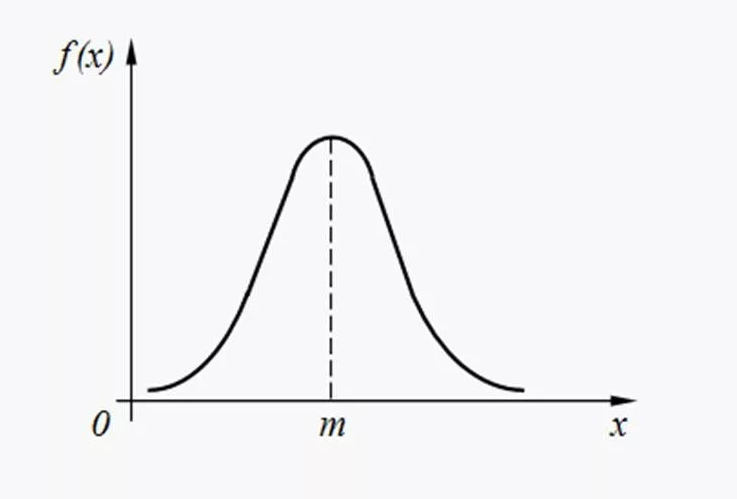
\includegraphics[width=0.5\textwidth]{image1.png}
    \caption{График распределения функции}
    \label{fig:first_graph}
\end{figure}

\begin{figure}[htbp]
    \centering
    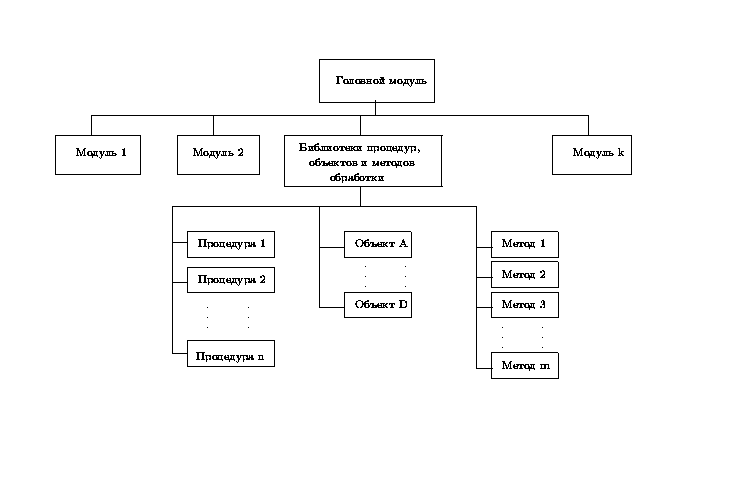
\includegraphics[width=0.5\textwidth]{image2.png}
    \caption{Структурная схема программного модуля}
    \label{fig:second_graph}
\end{figure}

Использование Docker-контейнеризации~\cite{docker-docs} позволяет изолировать выполнение данного программного кода.

% Заключение
\conclusion
В ходе выполнения отчётной работы были успешно решены задачи математического моделирования и обработки данных. Программный код на языке \texttt{C++} показал высокую эффективность. Использование системы \LaTeX{} совместно с шаблоном СГУ позволило оформить текстовый документ в строгом соответствии с установленными стандартами, автоматически связав формулы, таблицы, рисунки и библиографические источники.

% Библиографический список
\bibliographystyle{ugost2003}
\bibliography{thesis}

% Приложения (если необходимы, каждая последующая секция будет приложением)
\appendix

\end{document}